\documentclass[imperial, justified]{octavo}
\usepackage{caption}
\usepackage{natbib}
\usepackage{lstdoc}
\usepackage{lipsum}
\usepackage{graphicx}
\usepackage{overpic}
\usepackage{url}
\global\setlength\parindent{1em}
\newif\ifdebug
\debugfalse
\ifdebug  
  \setlength\fboxsep{1pt}
\else
  \setlength\fboxsep{0pt}
  \setlength\fboxrule{0pt}
\fi

%% temporary titles
% command to provide stretchy vertical space in proportion
\newcommand\nbvspace[1][1]{\vspace*{\stretch{#1}}}

% allow some slack to avoid under/overfull boxes
\newcommand\nbstretchyspace{\spaceskip0.5em plus 0.25em minus 0.25em}

% To improve spacing on titlepages
\newcommand{\nbtitlestretch}{\spaceskip0.6em}

% temporary length used for some tables
\newlength{\TmpLen}

\begin{document}
\clearpage
\pagestyle{empty}
\begin{center}
\bfseries

\nbvspace[1]
\Huge
{\nbtitlestretch\huge
 TYPESETTING  
WITH  \TeX\ AND SX.TX FRIENDS  \\
}

\nbvspace[2]
\normalsize
TO WHICH IS ADDED MANY USEFUL MACROS
AND CODE WRITTEN SO THAT HE WHO RUNS MAY HACK

\nbvspace[1]
\small BY\\
\nbvspace[1]
\Large THE STACKEXCHANGE COMMUNITY {\large\textsc{}}\\[0.5em]
%\footnotesize AUTHOR OF ``A WORKING ALGEBRA,'' ``WIRELESS TELEGRAPHY,\\
%ITS HISTORY, THEORY AND PRACTICE,'' ETC., ETC.

\nbvspace[4]

%\includegraphics[width=0.8in]{ejc.pdf}
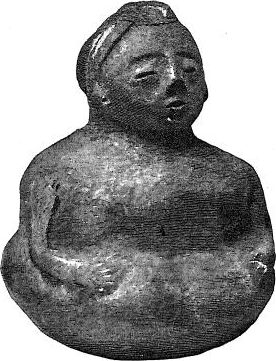
\includegraphics[width=1.5in]{./images/fig176}
\par
\nbvspace[2]
\normalsize
%DOHA$\cdot$BERLIN$ \cdot$ WILD

\nbvspace[10]
\Large
PUBLISHED IN THE WILD
%
\end{center}


\long\def\secondpage{\clearpage\null\vfill\vfill
\pagestyle{empty}
\begin{minipage}[b]{0.9\textwidth}
\footnotesize\raggedright
\setlength{\parskip}{0.5\baselineskip}
Copyright \copyright 2010--\the\year\ Dr Yiannis Lazarides\par
Permission is granted to copy, distribute and\slash or modify this document under the terms of the GNU Free Documentation License, version 1.2, with no invariant sections, no front-cover texts, and no back-cover texts.\par
A copy of the license is included in the appendix.\par
This document is distributed in the hope that it will be useful, but without any warranty; without even the implied warranty of merchantability or fitness for a particular purpose.
\end{minipage}
\vspace*{2\baselineskip}}

\secondpage

\backmatter
\tableofcontents
\listoffigures

\chapter{PREFACE}
This small booklet aims to describe some of the common problems encountered with the 
placement of figures in books. It also tries to provide techniques for storing them within TeX.

\mainmatter
\chapter{HOW TO TYPESET A LOT OF FIGURES}

\def\figurename{\textbf{Plate}}

If you have a lot of figures, it is a lot of work to have to maintain them, as well as
to remember all the file names

\section{A long table for figures}

We are familiar with longtable for tables, this is an equivalent technique for lots of figures.
\smallskip

\long\def\putgraphic#1{%
\fbox{%
\begin{minipage}[b]{2.0cm}%
 \centering
 \vspace{3.8pt}\fbox{%
 \includegraphics[width=0.98\textwidth,height=2.3cm,keepaspectratio]{./images/#1}}%
  \vspace{0.2cm} #1%\captionof{figure}\relax
  \vspace{0.2cm}%
  \end{minipage}}\hfil
}

\DeclareRobustCommand{\putcaption}[1]{\captionof{figure}{#1}}

\makeatletter
\def\alist{fig145,fig161,fig162,fig163,fig164,fig165,fig166,fig167,%
fig168,fig169,fig170,fig171,fig172,fig173,fig174,fig175,fig176,fig177,%
fig180,fig181,fig182,fig183,fig185,fig186,fig187,fig188,fig189}
\@for \i:=\alist\do{%
\expandafter\putgraphic{\i}% 
}
\putcaption{Weaving and pottery artifacts from Arizona.}

\section{More on figures and looping}

We can extend our macros and try and save some information for each image. To do this we
need to have a way to associate information with the figure number so we will create a number of commands
for each figure.

The \TeX\ way of defining commands on the fly that include non-letters is to use \verb+\csname+
\begin{verbatim}
\expandafter\def\csname fig170\endcsname#1{#1}
\@nameuse{fig170}{Pottery found in Apache%
    lands in Texas.}
\end{verbatim}
\@nameuse{fig170}{Pottery found in Apache %
    lands in Texas.}

This is not very useful, as it is. It is preferable to actually create a little command factory, that can create these
commands.

\begin{verbatim}
\def\commandfactory#1#2{
   \expandafter\def\csname #1\endcsname{#1}
   \expandafter\def\csname #1@caption\endcsname{#2}
}
\end{verbatim}
\def\commandfactory#1#2{
   \expandafter\def\csname #1\endcsname{#1}
   \expandafter\def\csname #1@caption\endcsname{#2}
}
\commandfactory{fig170}{Test}

\@nameuse{fig170@caption}


Since we are going to have to type a lot of information into a database to hold information for our images, we might as
well type it straight into our text.

Out of consideration for our users we may want to provide a short command for this.

\begin{verbatim}
\let\img\commandfactory
\end{verbatim}
\let\img\commandfactory

\img{fig171}{Testing again for something.}

We may also want to save the use of the curly brackets, that would visually distruct. We can redefine the Command factory to be a delimited macro. There is a lot of information on delimited macros. One of them is in such a place, hiding on \texttt{tex.sx}.

\def\commandfactory#1|#2|{
   \expandafter\def\csname #1\endcsname{#1}
   \expandafter\def\csname #1@caption\endcsname{#2}
}

\commandfactory fig172|This is figure 172|

\commandfactory fig173|This is figure 173|

\texttt{\@nameuse{fig172@caption}}

\texttt{\@nameuse{fig173@caption}}

Now that we have figured a way to define an efficient way to store information for our figures, we need to build some routines to sort them print them and other similar housekeeping routines.

\section{Sorting}

\global\setlength\parindent{1em}
I have still to find a better sorting routine other than the one available in the listings documentation. I did try my hands with LuaTeX but I am not very fond of jumping i and out of LaTeX. It can also create problems with updates and users that might not have LuaTeX installed.

We will store the record index in a macro that is essentially a comma delimited list. Don't be frighten about speed
I have used this method to store over 4000 figures and there was no problem either with the processing speed or with TeX'es memory.

We call this macro \verb+dbartifacts+, giving it a non-generic name. But first let us see, how we can add items in
and out of the macro. We start from an empty macro.

\begin{verbatim}
\def\dbartifacts{ }
\end{verbatim}
\let\dbartifacts\empty

We can use \LaTeX's \verb+\g@addto@macro+ to then add the items to the \verb+\dbartifacts+ macro.
\begin{verbatim}
\g@addto@macro{\dbartifacts}{fig172,}%
\g@addto@macro{\dbartifacts}{fig173,}%
\end{verbatim}

\g@addto@macro{\dbartifacts}{fig172,}%
\g@addto@macro{\dbartifacts}{fig173,}%


Testing it by just typing \verb+\texttt{\dbartifacts}+ we get: \texttt{\dbartifacts}. This of course is not very convenient and we would rather define a macro to save all the typing and have a more user friendly command.

\begin{verbatim}
\def\addtodb#1#2{%
  \g@addto@macro#1{#2,}%
}
\end{verbatim}
\def\addtodb#1#2{%
  \g@addto@macro#1{#2,}%
  \lst@BubbleSort\dbartifacts%
}

There are many other ways to manipulate the list, including using token registers, elt lists etc, but for such constructions as the ones described here, this is by far the simpler and the easiest.
We can now use this macro, when required:

\begin{verbatim}
\addtodb{\dbartifacts}{fig170}%
\addtodb{\dbartifacts}{fig171}%
\end{verbatim}

Testing again we get \texttt{\dbartifacts} an as you can see it works nicely. This method of trying out your code bit by bit, I call the water painting technique. So now that we have almost got all the routines we want, we can now look at sorting. This we achieve by adding \verb+ \lst@BubbleSort\dbartifacts+. Every time we add a record, the file will be sorted. Intuituitevely, this might not  be very efficient, especially if you are adding a lot of records at one time, but we can add more helper routines later for this.

\begin{verbatim}
\def\addtodb#1#2{%
  \g@addto@macro#1{#2,}%
  \lst@BubbleSort\dbartifacts%
}
\end{verbatim}

\def\figurename{\textbf{Figure}}
\begin{figure}
\vspace*{1cm}
\centering
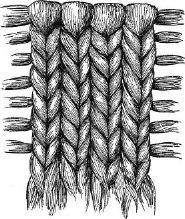
\includegraphics[scale=0.6]{./images/fig172}
\caption{Textiles from Arizona. }
\end{figure}

\section{Adding some more user helper macros}

It is expected that the user will produce a file, either through some automatic means or by typing it to hold the data. Deletion and insertion is simply via editing this file through a text editor. However, for completeness, we will write a few macros to help with maintenace of the database. These include macros for delete and modify record etc.

Another set of macros that one can use is to typet the records in lists and or tabulat forms, if required. Early books on archaelogy for example listed all the items in the following format, interspersed with comments and figures.
\smallskip


\hangindent3em
2520. (39510). A double globe jar or canteen. White ground, with ornamentations in black, as seen in Fig. 649. Depression in the center is probably designed to receive a band or cord to carry it with.
\smallskip

Although one is tempted to produce a list for these, the next item from such a book points otherwise:
\smallskip

\hangindent3em
2677-2678. 2677, (39617), and 2678, (39618). With flared and notched rim.
\smallskip

Before extending the database for such forms of descriptions, we can develop the typesetting part. I am sure that Lamport would have used a list, possibly due memory and space limitations and just re-use the \verb+\item+ command, in our case it is better to rather define a small macro
to cater for such items. The indentation can easily be achieved using \verb+\hangindent3em+ or a similar amount of measure.

\begin{verbatim}
\long\def\catno#1\par{
\par%
\hangindent3em\noindent
#1
}
\end{verbatim}


\def\catno#1#2{%
    \@hangfrom{#1. }#2
}

\LaTeX\ provides a macro named \verb+\@hangfrom{<text>}+, that puts $<text>$ in a box, and makes a hanging indentation of the following material up to the firrst \verb+\par+. Should be used in vertical mode.\footnote{See source2e, \texttt{ltsect.dtx}, pg 287.}

\begin{verbatim}
121 \def\@hangfrom#1{\setbox\@tempboxa\hbox{{#1}}%
122 \hangindent \wd\@tempboxa\noindent\box\@tempboxa}
\end{verbatim}

\medskip

\catno{289}{(39914). Fig. 397. Red ware, with white lines on the lower globe and decorations in black on the upper, with orifice in each globe.}

\catno{1289}{(39914). Fig. 397. Red ware, with white lines on the lower globe and decorations in black on the upper, with orifice in each globe.}


\makeatother

\section{Epiloque}

We have managed to write a database, sort it, typeset its contents in a structured or freeform manner
and on the way we have documented the code using a form of \textit{literate programing.} On top which
other language expects you to code your own ifs and for? 
The amount of code we wrote was very minimal and competes well with modern computer languages. 
Hope you had fun. Go and make beautiful books. \citet{knuth98}


%
%\chapter{The full listing}
%\centering
%\begin{overpic}[grid,scale=0.5,unit=1mm]%
%{./images/fig198}
%\put(3,92){\color{red}\huge \LaTeX}
%\end{overpic}


 \subsection{Acknowledgements}

 Octavo is a modification of \texttt{classes.dtx} written by Leslie Lamport (1992),
 Frank Mittelbach (1994-97) and Johannes Braams (1994-97). As can be seen
 from the code, my own input is restricted to a tweaking of some parameters
 and true credit is due to Lamport, Mittelbach and Braams for their
 monumental efforts.

 \begin{thebibliography}{16}

 \bibitem{knuth98} Knuth,~D. 1998. \emph{Digital Typography}. CSLI 
 Publications, Stanford.

 \bibitem{rosarivo61} Rosarivo,~R. 1961. \emph{Divina proportio typographica}. 
 Scherpe, Krefeld.

 \bibitem{taylor98} Taylor,~P. 1998. \emph{Book design for \TeX\ users, Part 1: 
 Theory.} TUGBoat, 19:65--74.

 \bibitem{taylor99} Taylor,~P. 1999. \emph{Book design for \TeX\ users, Part 2:
 Practice.} TUGBoat, 20:378--389.

 \bibitem{town} Town,~L. \emph{Bookbinding by hand.} Faber \& Faber, London.

 \bibitem{tschichold87} Tschichold,~ J. 1987. \emph{Ausgew\"{a}hlte Aufs\"{a}tze
 \"{u}ber Fragen der Gestalt des Buches und der Typographie}. Birkh\"{a}user
 Verlag, Basel.

 \bibitem{williamson66} Williamson,~H. 1966. \emph{Methods of book design.} Oxford 
 University Press, Oxford.

 \bibitem{wilson01} Wilson,~P. 2001. \emph{The Memoir class for configurable
 typesetting.} CTAN. \url{macros\\latex\\contrib\\memoir} 

 \end{thebibliography}




\end{document}